La gestión de paquetes consiste en el conjunto de herramientas que permiten descargar y mantener las dependencias que el proyecto va a utilizar. Como se ha decidido utilizar React + Express, el entorno de desarrollo es todo Javascript y, por tanto, en servidor se va a utilizar NodeJS, que tiene su propio gestor de paquetes: NPM.

Aunque NPM es una herramienta muy útil en su campo, no es la única que se ha creado para este propósito. Y hoy por hoy, la herramienta competidora por excelencia es Yarn. Como bien explica \citet{NPMVYRN}, existe una diferencia de velocidad a favor de Yarn (ver figura \cref{fig:package-manager:middle-size}). Sin embargo, \citet{NPMVYRN} también nos dice que esa diferencia de velocidad no es grande, así que no debería ser el motivo para elegir un gestor u otro. La funcionalidad de ambos gestores, pese a ser similar, tiene sus diferencias. Además, Yarn sacrifica espacio en disco para ganar ese extra de velocidad que NPM no tiene.

Como en este punto la decisión es tremendamente subjetiva y el coste de implementar ambos es pequeño, para este proyecto me voy a tomar la molestia de contemplar ambas opciones a la vez. Esto quiere decir que, en la configuración inicial del entorno, se presupondrá NPM (que es el gestor por defecto de Node), pero se permitirá al usuario cambiar a Yarn de forma sencilla y rápida.

\begin{figure}
	\centering
	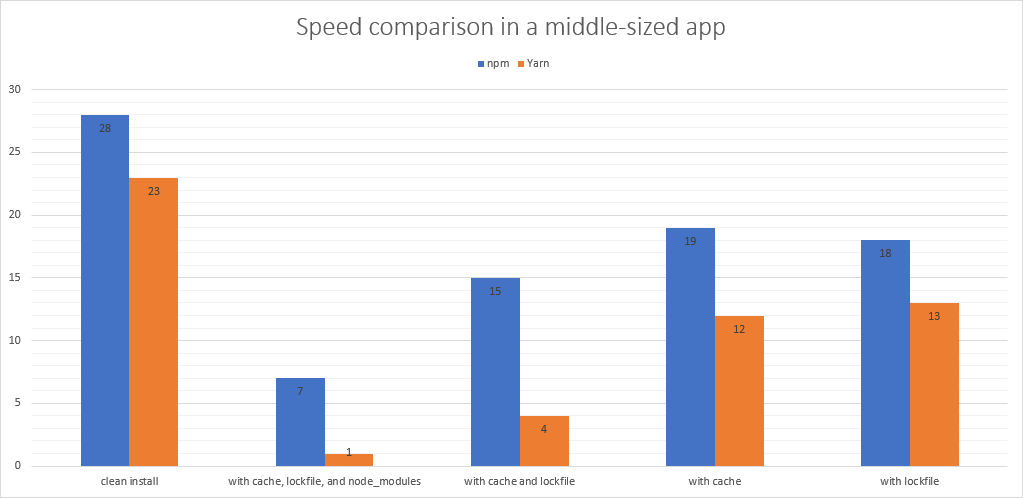
\includegraphics[width=\textwidth]{yarn-vs-npm-middle-sized-apps.jpg}
	\caption{NPM vs Yarn. Speed comparison in a middle-sized app}
	\label{fig:package-manager:middle-size}
\end{figure}
